\documentclass[11pt]{article}
\usepackage{latexsym}
\usepackage{natbib}
\usepackage{graphicx}
\usepackage{subfigure}
\usepackage{listings}
\usepackage{algorithm}
\usepackage{algpseudocode}

\title{Homework 4: Approximate Inference in Bayesian Networks}
\author{Shun Zhang}
\date{}

\begin{document}
\maketitle

\section{Introduction}

\begin{equation}
p(x_i|x_{\{j \not = i\}}) \propto \prod_k P(x_k|pa_k)
\end{equation}

% \begin{figure}
% \centering
% 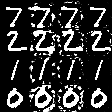
\includegraphics[]{test.png}
% \caption{Reconstruction of digits. From left to right on each line,
% there are original digits, digits constructed by first 100
% eigenvectors, digits constructed by first 200 eigenvectors, and digits
% constructed by first 600 eigenvectors. }
% \label{fig:test}
% \end{figure}

\end{document}
